\chapter{The \acl{SM}}
\label{chap:intro:sm}

The \acf{SM} is a quantum field theory that describes the interactions of three 
of the four fundamental forces of nature, electromagnetism, the weak force, and 
the strong force, with a set of fundamental particles.
The \ac{SM} makes many predictions, from the spectral lines of the hydrogen  
atom to the rate of the \BsTomumu\ decay, and so far no experimental results 
have provided conclusive proof that such predictions are, fundamentally, 
incorrect.
The absence of a description of the fourth fundamental force, gravity, the 
non-zero masses of neutrinos, and several astronomical observations indicate 
that, at the very least, the \ac{SM} is not a complete description of the 
universe.
It does not describe the observed matter-antimatter asymmetry, nor can it 
account for the apparent presence of dark matter.
The purpose of the \ac{LHC} is to provide experiments with enough data to be 
able to find minute deviations from the predictions of the \ac{SM}, which could 
point to particular extensions of theory.
In this \lcnamecref{chap:intro:sm}, the forces and particles described by the 
\ac{SM} are summarised.
Particular emphasis is given to the phenomenology of the weak force, which the 
\lhcb\ detector is optimised to study.

The \ac{SM} is a powerful predictive model partly due to its use of symmetries, 
which, through Noether's theorem, give rise to conserved currents.
For example, the symmetry of physical laws to rotations in space and 
translations in time leads to the conservation of total angular momentum and 
energy, respectively.
In a quantum field theory, each of these currents are quantised in units of a 
quantum charge.
Interactions with a field only occur if the particles are charged under that 
field, such as the familiar electric charge for the electromagnetic field, and 
all interactions conserve the total charge of the system.

Interactions with fields are mediated via the exchange of bosons, particles 
with integer spin, such as the photon, the force carrier of the electromagnetic 
field.
Fermions are particles with half-integer spins; the quarks, leptons, and 
neutrinos constitute the fundamental fermions.
The projection of a particle's spin vector along its momentum vector defines 
the particle's helicity, and is not invariant under Lorentz transformations.
The chirality of a particle can be considered as a Lorentz invariant helicity, 
as such encoding the intrinsic `handedness' of a particle.
The known fundamental particles of the \ac{SM}, along with their measured 
electric charges and spins, are shown in \cref{tab:intro:sm:particles}.

\begin{table}
  \centering
  \caption{%
    Properties of the fundamental particles of the \acl{SM}~\cite{PDG2014}. The
    electric charge is given in units of the electron charge.
  }
  \label{tab:intro:sm:particles}
  \begin{tabular}{cccc}
  \toprule
  Particle                    & Electric charge & Spin         & Mass (\si{\GeVcc})         \\
  \midrule
  \Pup, \Pcharm, \Ptop        & \sfrac{2}{3}    & \sfrac{1}{2} & \num{2.2e-3}, $1.3$, $173$ \\
  \Pdown, \Pstrange, \Pbottom & $-\sfrac{1}{3}$ & \sfrac{1}{2} & \num{4.7e-3}, $0.1$, $4.2$ \\
  \Pelectron, \Pmuon, \Ptau   & $-1$            & \sfrac{1}{2} & \num{0.5e-3}, $0.1$, $1.8$ \\
  \Pnue, \Pnum, \Pnut         & $0$             & \sfrac{1}{2} & $> 0$                      \\
  \midrule
  \Pphoton                    & 0               & 1            & 0                          \\
  \Pgluon                     & 0               & 1            & 0                          \\
  \PWp                        & $\pm1$          & 1            & $80.4$                     \\
  \PZ                         & 0               & 1            & $91.2$                     \\
  \PH                         & 0               & 0            & $125$                      \\
  \bottomrule
\end{tabular}

\end{table}

The strong force acts on particles with colour charge, quarks and gluons, via 
the exchange of gluons.
The fact that gluons are charged under the force they mediate significantly 
complicates the theory of strong interactions.
At low energies, the self interaction leads to the phenomenon of confinement, 
whereby free colour-charged objects cannot be observed, as the attractive force 
between two colour-charged objects is approximately constant at large 
separations, and so an infinite amount of energy is required to separate such 
objects completely.
Conversely, at higher energies, these particles become asymptotically free, 
eventually forming a quark-gluon plasma.
The energy scale at which the transition between these two regimes occurs is 
denoted \qcdscale.

Theoretical studies of the strong force use the framework of \ac{QCD}, which 
can either be used perturbatively, when the energy scale of the process under 
consideration is much larger than \qcdscale, or non-perturbatively, when the 
opposite is true.
It is feasible to make predictions using perturbative \ac{QCD}, although the 
computations become more challenging as the order in the perturbative 
expansions increases.
Predictions requiring non-perturbative \ac{QCD} are generally not possible to 
perform analytically with today's understanding, although lattice \ac{QCD} can 
offer an alternate means of computation for some problems.
In most cases, experimental input is necessary to constrain the theory.
One such example of a non-perturbative problem is the prediction of \pp\ 
cross-sections at the \ac{LHC}, which will be discussed in more detail in 
\cref{chap:prod:theory}.

Through confinement, the six quarks (\Pup, \Pdown, \Pcharm, \Pstrange, \Ptop, 
and \Pbottom) cannot be observed as free states.
The five lightest quarks bind together to form hadrons, colourless states of 
two or more quarks bound together with a `sea' of gluons.
The top quark decays too quickly to form such states.
When quarks and gluons act as outgoing objects in interactions, the observed 
final state is a shower of colourless particles, each formed through the 
process of hadronisation, where the initial quark or gluon `fragments' into 
additional coloured objects.

Mesons are hadrons comprising a quark-anti-quark pair, and baryons contain 
three quarks or three anti-quarks.
More exotic states, such as tetra- or penta-quarks, also 
exist~\cite{Choi:2007wga,Aaij:2014jqa,Aaij:2015tga}, but have not been observed 
outside of particle collider experiments.
The behaviour of hadrons can be studied with a particle detector to infer the 
behaviour of the quarks and gluons.
In particular, the \lhcb\ detector is optimised to select and reconstruct the 
decays of mesons and baryons containing \Pcharm and \Pbottom quarks, in order 
to probe the nature of the weak force.
These include the charm mesons \PDzero~($\Pcharm\APup$) and 
\PDp~($\Pcharm\APdown$), beauty mesons \PBzero~($\Pdown\APbottom$) and 
\PBp~($\Pup\APbottom$), and the charm and beauty baryons 
\PLambdac~($\Pup\Pdown\Pcharm$) and \PLambdab~($\Pup\Pdown\Pbottom$).
The decays of these hadrons to sets of comparatively long-lived particles, such 
as charged pions~($\Pup\APdown$) and kaons~($\Pup\APstrange$), 
protons~($\Pup\Pup\Pdown$), and leptons, allow the properties of the heavy 
flavour hadrons to be inferred through the interactions of the decay products 
with the detector.\footnotemark\
\footnotetext{%
  Throughout this thesis, charge conjugation is implied unless stated 
  otherwise.
}

% and the carriers are the two charged \PWpm bosons and the neutral \PZ boson.

The weak force interacts with particles with a left-handed chirality and with a 
non-zero weak isospin \wisospin.
The symmetry under the parity transformation \Ptransform, which changes the 
sign of the spatial coordinates, is maximally violated by the weak force only 
coupling to left-handed particles.
The discovery of \Ptransform\ violation~\cite{Wu:1957my} was soon followed by 
the discovery of \CP\ violation~\cite{Christenson:1964fg}, the breaking of the 
symmetry of the \CP\ transformation which simultaneously changes the handedness 
of particles (\Ptransform) and transforms particles into their anti-particles.  
(\Ctransform).

The weak force is particularly interesting to study because it is the only 
force to have been observed to break the \Ptransform\ and \CP\ symmetries.
In addition, at high energies the weak field unifies with the electromagnetic 
field to form the electroweak field.
Prior to the process of electroweak symmetry breaking, where the two component 
fields become physically distinguishable, the electroweak field has four 
massless degrees of freedom.
After this, two degrees of freedom are observed experimentally as the massive 
\PWp and \PWm bosons, whereas the other two degrees of freedom, $\PW^{0}$ and 
$\PB^{0}$, mix to form the observed massive \PZ boson and the massless photon.
The `spontaneous' breaking of the electroweak unification at low energies is 
caused by the so-called Higgs mechanism, wherein an additional field, the Higgs
field, contributes four additional degrees of freedom to the theory.
Three degrees of freedom of the Higgs field mix with three degrees of freedom 
of the electroweak field to give masses to the \PWpm and \PZ bosons, whilst the 
fourth degree of freedom can be interpreted a new boson \PH, the Higgs 
particle.

The study of the Higgs particle has only become possible with the \ac{LHC}, at 
which the Higgs boson was discovered by the \atlas\ and \cms\ 
collaborations~\cite{Aad:2012tfa,Chatrchyan:2012xdj}.
Studies continue to measure the properties of the 
Higgs~\cite{Khachatryan:2016vau}, to see whether it behaves in a way predicted 
by the \ac{SM}.
Deviations in the behaviour of this particle can indicate the presence of 
particles not predicted by the \ac{SM}, observations of which would be 
considered a major breakthrough in high energy physics.
Observations of large \CP-violating effects would be of similar interest, but 
can relate to different phenomena.

\section{\texorpdfstring{\CP}{CP} violation}
\label{chap:intro:sm:cp}

As the measurement of \CP\ violation in charm and beauty hadron decays is a 
cornerstone of the \lhcb\ physics programme, and indeed of \cref{chap:cpv} of 
this thesis, its mechanism will be describe here in more detail.

The weak interaction eigenstates $(\Pdown', \Pstrange', \Pbottom')$ are 
different to the quark mass eigenstates $(\Pdown, \Pstrange, \Pbottom)$.
The weak eigenstates are a superposition of the mass eigenstates, the linear 
coefficients of which are given by the \ac{CKM} matrix
\begin{equation}
  \begin{pmatrix} \Pdown' \\ \Pstrange' \\ \Pbottom' \end{pmatrix}
  =
  V_{\text{CKM}}\begin{pmatrix} \Pdown \\ \Pstrange \\ \Pbottom \end{pmatrix}
  =
  \begin{pmatrix}
    \Vud & \Vus & \Vub \\
    \Vcd & \Vcs & \Vcb \\
    \Vtd & \Vts & \Vtb
  \end{pmatrix}
  \begin{pmatrix} \Pdown \\ \Pstrange \\ \Pbottom \end{pmatrix},
\end{equation}
where $V_{ij}$ is the coupling of the $i$ to $j$ transition, e.g.\ $|\Vud|^{2}$ 
is the relative probability of the transition \decay{\Pdown}{\Pup}.
The values of the \ac{CKM} matrix elements are not predicted by the \ac{SM} and 
so must be determined experimentally.
There are several methods for determining the coupling constants, depending on 
the quarks involved, but each generally involves the measurement of one or more 
decay rates involving a particular quark transition, and require some 
theoretical input to disentangle the contributions from the strong and weak 
forces.
One example measurement is $\beta$ decay, used as input to compute \Vud.
Given that the up and down quarks are the most abundant, \Vud\ is particularly 
well known, with a fractional uncertainty of the order of \num{e-5}.
The element \Vub\ is the least well known, with a fractional uncertainty around 
\SI{2}{\percent}, measured using the decays of beauty 
hadrons~\cite{Charles:2004jd}.

By exploiting the predicated unitarity of the \ac{CKM} matrix, it can be 
represented using only three mixing angles and a complex phase $\delta$
\begin{equation}
  V_{\textrm{CKM}} =
  \begin{pmatrix}
    c_{12}c_{13} & s_{12}c_{13} & s_{13}e^{-i\delta} \\
    -s_{12}c_{23} - c_{12}s_{23}s_{13}e^{-i\delta} & c_{12}c_{23} - 
    s_{12}s_{23}s_{13}e^{-i\delta} & s_{23}c_{13} \\
    s_{12}c_{23} - c_{12}c_{23}s_{13}e^{-i\delta} & -c_{12}s_{23} - 
    s_{12}c_{23}s_{13}e^{-i\delta} & c_{23}c_{13}
  \end{pmatrix},
\end{equation}
where $s_{ij} = \sin{\theta_{ij}}$ and $c_{ij} = \cos{\theta_{ij}}$.
In alternative formulations~\cite{Wolfenstein:1983yz}, the three angles are 
parameterised as $\alpha$, $\beta$ and $\gamma$ and can be visualised as a 
triangle on the complex plane.
One of the key measurements of \lhcb\ is that of the angle $\gamma$, which is 
the least well-measured of the three angles, with the precision on the world 
average around \SI{9}{\percent}~\cite{LHCb-CONF-2016-001}.
This is to be compared with the ultimate precision that could be obtained given
the finite uncertainty of some of the theoretical inputs, required to translate
the measurements into estimates of the CKM elements, estimated to be up to 
\SI{4}{\degree}, depending on the assumptions~\cite{Brod:2013sga,Brod:2014bfa}.

The closure of the $(\alpha, \beta, \gamma)$ triangle is equivalent to the 
prediction of the unitarity of the CKM matrix, and hence measuring a value of 
$\gamma$ which does not form a triangle would be a sign of physics beyond the 
\ac{SM}.
The current world averages of the various measurements are presented in the 
complex plane in \cref{fig:intro:sm:ckm_angles}, where some of experimental 
inputs and their associated uncertainties are shown as bands.
The \lhcb\ experiment has performed measurements of most of the inputs shown, 
with the exception of $\varepsilon_{\PK}$ which is related to neutral kaon 
oscillations.

It is the phase in the \ac{CKM} matrix that permits \CP\ violation.
Consider a decay \decay{P}{f} and the \CP\ conjugate process
\decay{\bar{P}}{\bar{f}}.
The corresponding decay amplitudes $\mathcal{M}_{f}$ and 
$\bar{\mathcal{M}}_{\bar{f}}$ can have some phase $\phi$, and the \ac{CKM} 
mechanism can add an additional phase $\theta$ which changes sign under \CP, 
giving
\begin{equation}
  \mathcal{M}_{f}             = |a| e^{i(\phi + \theta)}, \quad
  \bar{\mathcal{M}}_{\bar{f}} = |a| e^{i(\phi - \theta)},
  \label{eqn:intro:sm:weak:amplitudes_one}
\end{equation}
where $|a|$ is the magnitude of matrix element.
The observable rates of these processes, $|M_{f}|^{2}$ and 
$|\bar{M}_{\bar{f}}|^{2}$, are equal, and so the decay is symmetric under 
\CP\@.
However, for a process that can proceed via two channels, for example, such as 
in \cref{fig:intro:sm:weak_feynman}, the total matrix elements are 
$\mathcal{M}_{f} = \mathcal{M}_{f,1} + \mathcal{M}_{f,2}$ and 
$\bar{\mathcal{M}}_{\bar{f}} = \bar{\mathcal{M}}_{\bar{f},1} + 
\bar{\mathcal{M}}_{\bar{f},2}$ with
\begin{align*}
  \mathcal{M}_{f,1} &= |a_{1}| e^{i(\phi_{1} + \theta_{1})}, &
  \mathcal{M}_{f,2} &= |a_{2}| e^{i(\phi_{2} + \theta_{2})},\\
  \bar{\mathcal{M}}_{\bar{f},1} &= |a_{1}| e^{i(\phi_{1} - \theta_{1})}, &
  \bar{\mathcal{M}}_{\bar{f},2} &= |a_{2}| e^{i(\phi_{2} - \theta_{2})}.
\end{align*}
It then follows that
\begin{equation*}
  |\mathcal{M}_{f}|^{2} - |\bar{\mathcal{M}}_{\bar{f}}|^{2} =
  -4|\mathcal{M}_{1}||\mathcal{M}_{2}|\sin(\phi_{1} - \phi_{2})\sin(\theta_{1} 
  - \theta_{2}).
\end{equation*}
This is non-zero, provided that $\theta_{1} \neq \theta_{2}$ and $\phi_{1} \neq 
\phi_{2}$, and hence introduces a possible \CP\ asymmetry.
It is then the interference between channels that permits \CP\ symmetry 
breaking in weak interactions.

The breaking of the \CP\ symmetry was first observed in kaon decays in 
1964~\cite{Christenson:1964fg}, and in 2001 \CP\ violation was first observed 
in beauty decays~\cite{Aubert:2001nu,Abe:2001xe}.
Observing \CP\ violation in charm decays would provide a more complete picture 
of what is possible in the \ac{SM}, but it will not solve the problem of the 
observed baryon asymmetry in the universe, which the \ac{SM} cannot account 
for.
In the \ac{LHC} era, it is hoped that signs of physics \acl{BSM} will point to 
specific, new theories, that themselves may have explanations for this great 
mystery.

\begin{figure}
  % The relative widths of the subfigures here have been
  % roughly tweaked to produce equally sized fonts
  \begin{subfigure}{0.40\textwidth}
    \centering
    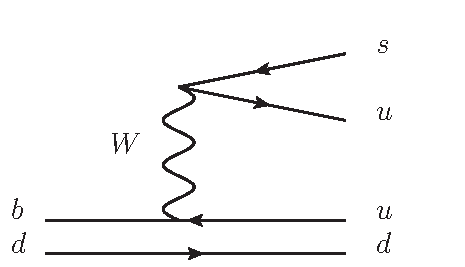
\includegraphics[width=\textwidth]{introduction/weak_tree}
    \caption{Tree diagram}
    \label{fig:intro:sm:weak_feynman:tree}
  \end{subfigure}
  \begin{subfigure}{0.55\textwidth}
    \centering
    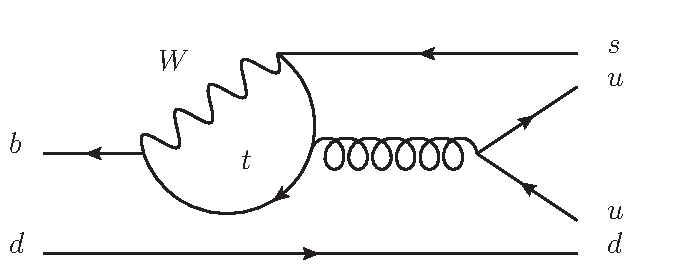
\includegraphics[width=\textwidth]{introduction/weak_penguin}
    \caption{Penguin diagram}
    \label{fig:intro:sm:weak_feynman:penguin}
  \end{subfigure}
  \caption{%
    Two possible Feynman diagrams for the decay \decay{\PBzero}{\PKplus\Ppiminus}.
  }
  \label{fig:intro:sm:weak_feynman}
\end{figure}

\begin{figure}
  \centering
  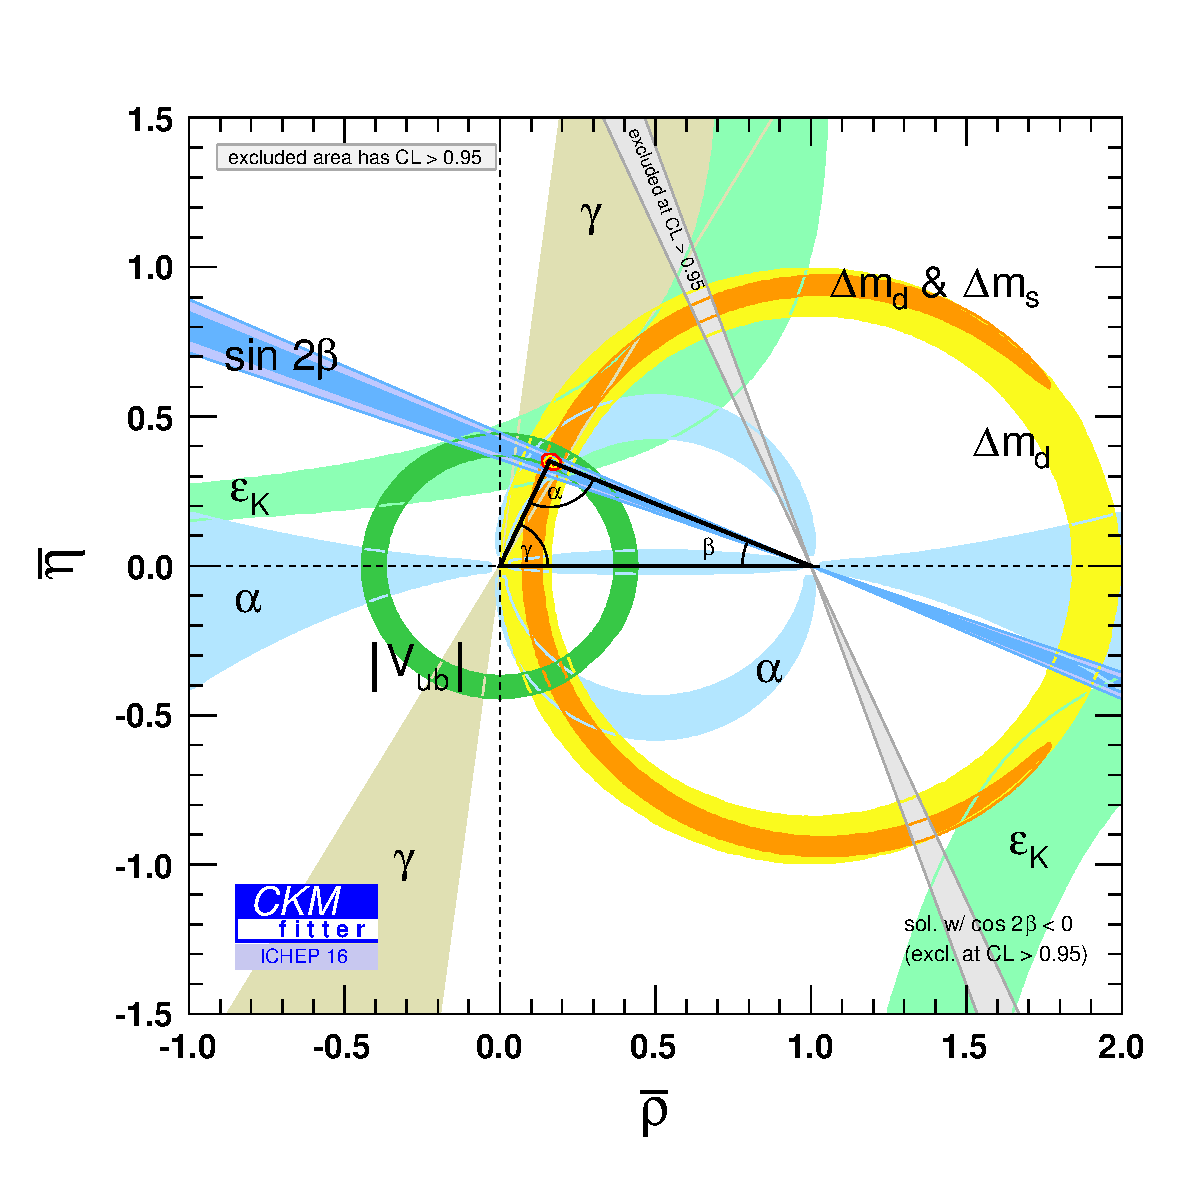
\includegraphics[width=\textwidth]{introduction/ckmfitter_rho_eta_plane}
  \caption{%
    A representation of the three angles, parameterised as $\alpha$, $\beta$, 
    and $\gamma$, of the CKM matrix shown the complex plane.
    The various bands show the experimental inputs to the determination of the 
    angles, with the width of the bands corresponding to the uncertainties on 
    the measurements.
    The angles and the measurements correspond to the world averages as of 
    mid-2016~\cite{Charles:2004jd}.
  }
  \label{fig:intro:sm:ckm_angles}
\end{figure}
